% -----------------------------*- LaTeX -*------------------------------
\documentclass[12pt]{report}
\usepackage{scribe}
\usepackage{hyperref}

% citation
\usepackage[authoryear]{natbib}
\bibliographystyle{abbrvnat}

% insert image
\usepackage{graphicx}

% cpation
\usepackage{caption}

% algorithm
\usepackage{algorithm}
\usepackage{algorithmicx}
\usepackage{algpseudocode}


% new command
\newcommand{\grad}{\nabla}
\newcommand{\curly}[1]{\left\{#1\right\}}
\newcommand{\notate}[1]{\text{#1\thinspace}}

\begin{document}
\scribe{Charles Kwong}
\lecturenumber{15}			% required, must be a number
\lecturedate{10/25}		% required, omit year

\maketitle

\framebox[.95\textwidth]{\parbox{.93\textwidth}{ {{\bf Note:}} These
lecture notes are still rough, and have only have been mildly proofread.  }}
\vspace*{.1in}


% ----------------------------------------------------------------------

\section{Introduction}
In this lecture, we will talk about scalable Stochastic Gradient Descent (SGD) algorithms. Many machine learning problems that we have visited so far can be solved in \emph{polynomial time}. However, in a big data analytics setting, where the sample size of the data, i.e.~$n$, can be astronomically large, and the dimension of the data, i.e.~$d$, can be intimidatingly high, polynomial time \emph{solvability} does not necessarily imply \emph{scalability}. 

A scalable algorithm hence must be fast. Ideally, the desirable time complexity should be linear with respect to $n$ and $d$, i.e.
\begin{equation*}
t = O(nd).
\end{equation*}
Furthermore, a scalable algorithm must also be easily \emph{parallelizable}, with a decreasing time complexity as the number of cores, $p$, available increases. i.e.~suppose a serial version of the algorithm runs in time $T$, a parallel version ran by $p$ cores should ideally have time complexity:
\begin{equation*}
t = O(T/p).
\end{equation*}

Last but by no mean the least, it goes without saying that the central goal of a scalable algorithm is to deliver an \emph{accurate} solution to the problem of interest. Among accuracy, speed, and parallelizability, machine learning practitioners evaluate the performance of the algorithms measured by these three criteria, as illustrated in Figure~\ref{fig:tradeoff}.

\begin{figure}
\centering
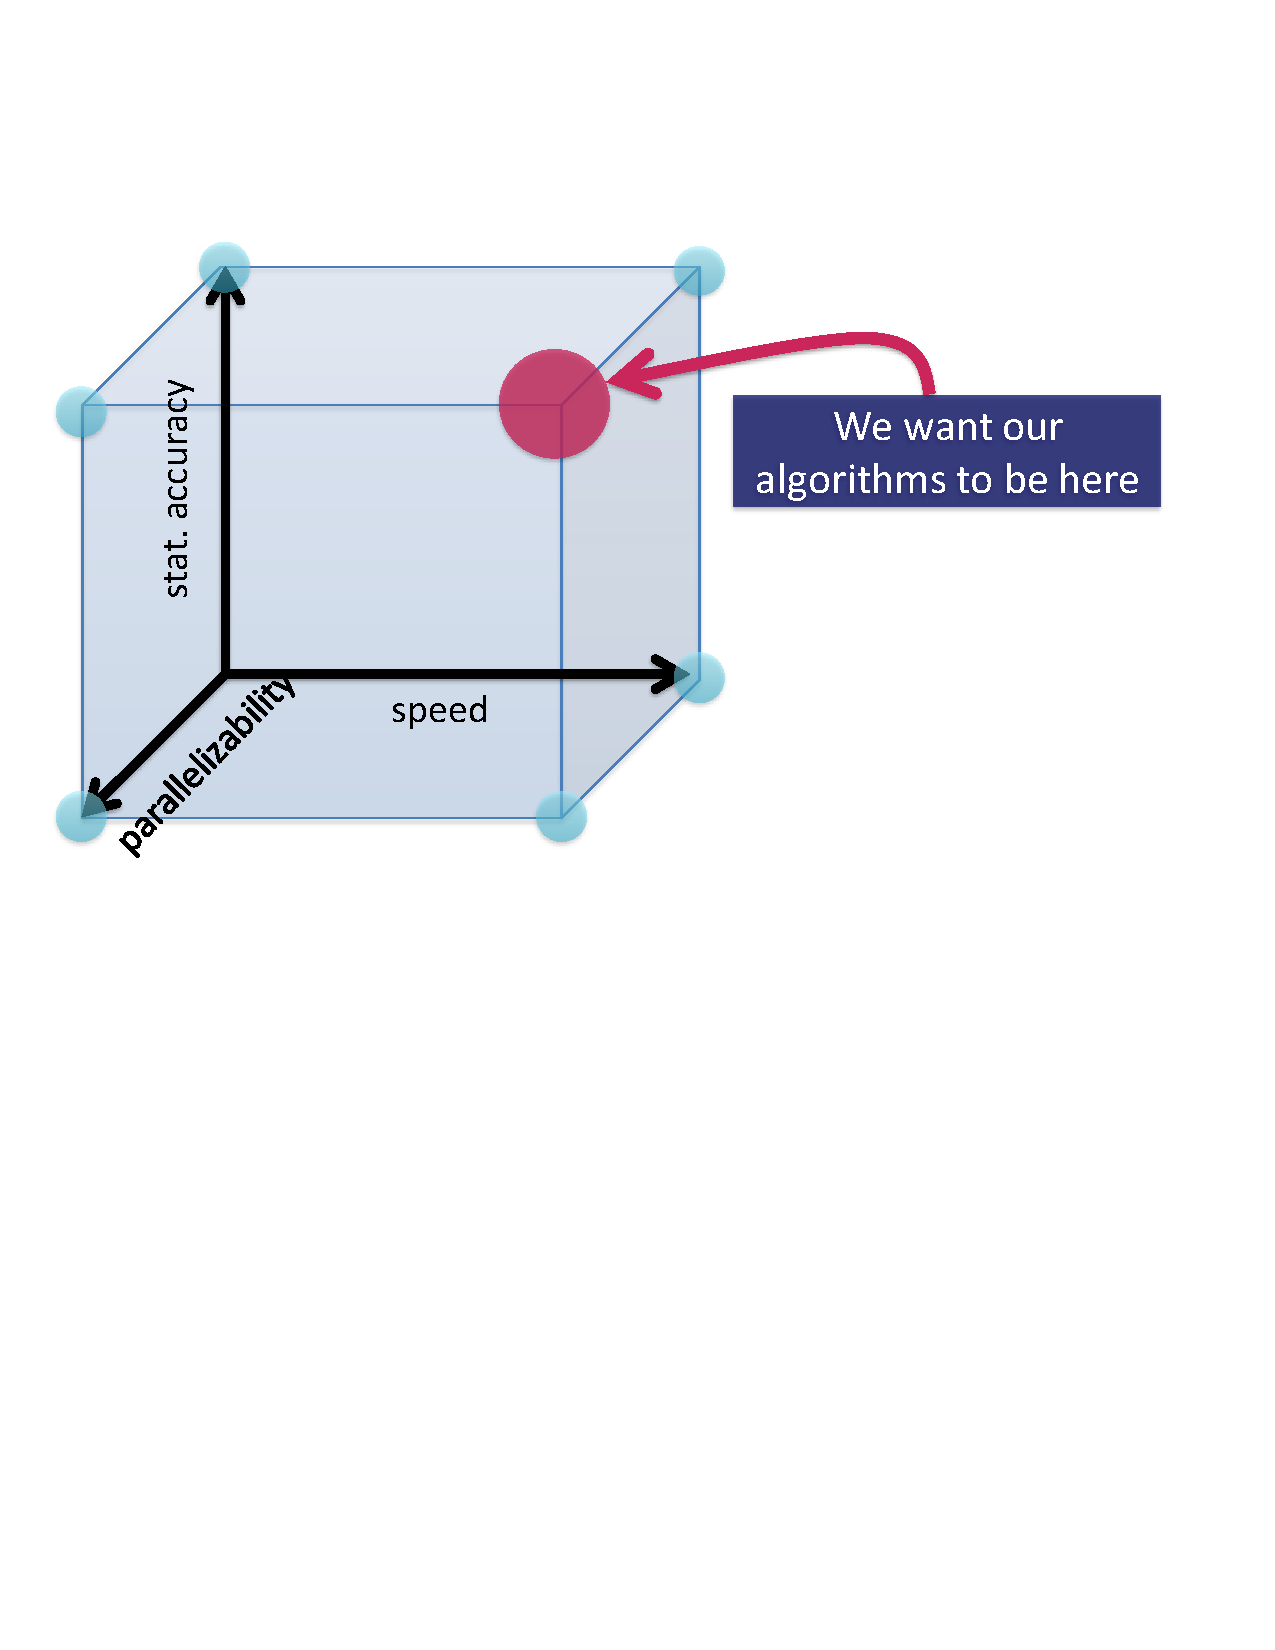
\includegraphics[scale=0.5]{./support/tradeoff.pdf}
\captionof{figure}{Performance Trade-off of a Machine Learning Algorithm}
\label{fig:tradeoff}
\end{figure}

\section{Stochastic Gradient Descent}
\label{sec:sgd}
Stochastic Gradient Descent (SGD) algorithm is an attractive option for solving many of the important machine learning problems, such as matrix completion, topic modeling, spectral analysis, graph clustering, perceptron learning, neural network (back propagation), principal component analysis (Oja's iteration), and least mean square filter. In many learning scenarios, SGD can deliver accurate solutions efficiently. Furthermore, SGD also demonstrates many desirable theoretical and empirical properties such as robustness to noise, simple implementation, small computational footprints, and stability. Let $x$ denote the parameterizaiton of a learning problem, SGD solves the following optimization problem,
\begin{equation*}
\arg\min_{x\in\mathbb{R}^d} \sum_{i=1}^n f_i(x),
\end{equation*}
where $f_i(x)$ is the value of a loss function that is only dependent on the $i^{th}$ data point of the dataset. At iteration $k$, suppose $x_k$ is available, the update rule of SGD is given by:
\begin{equation*}
x_{k+1} = x_k - \gamma_k \grad f_{s_k} (x_k),
\end{equation*}
where $\gamma_k > 0$ is the step length parameter, $\grad f_{s_k} (x_k)$ is the gradient of $f_{s_k} (x_k)$, and $s_k \in \curly{1,2,\cdots,n}$ is an index randomly drawn at the $k^{th}$ iteration in order to determine the data point on which the loss function and its gradient will be evaluated at the $k^{th}$ iteration.


\begin{figure}
\centering
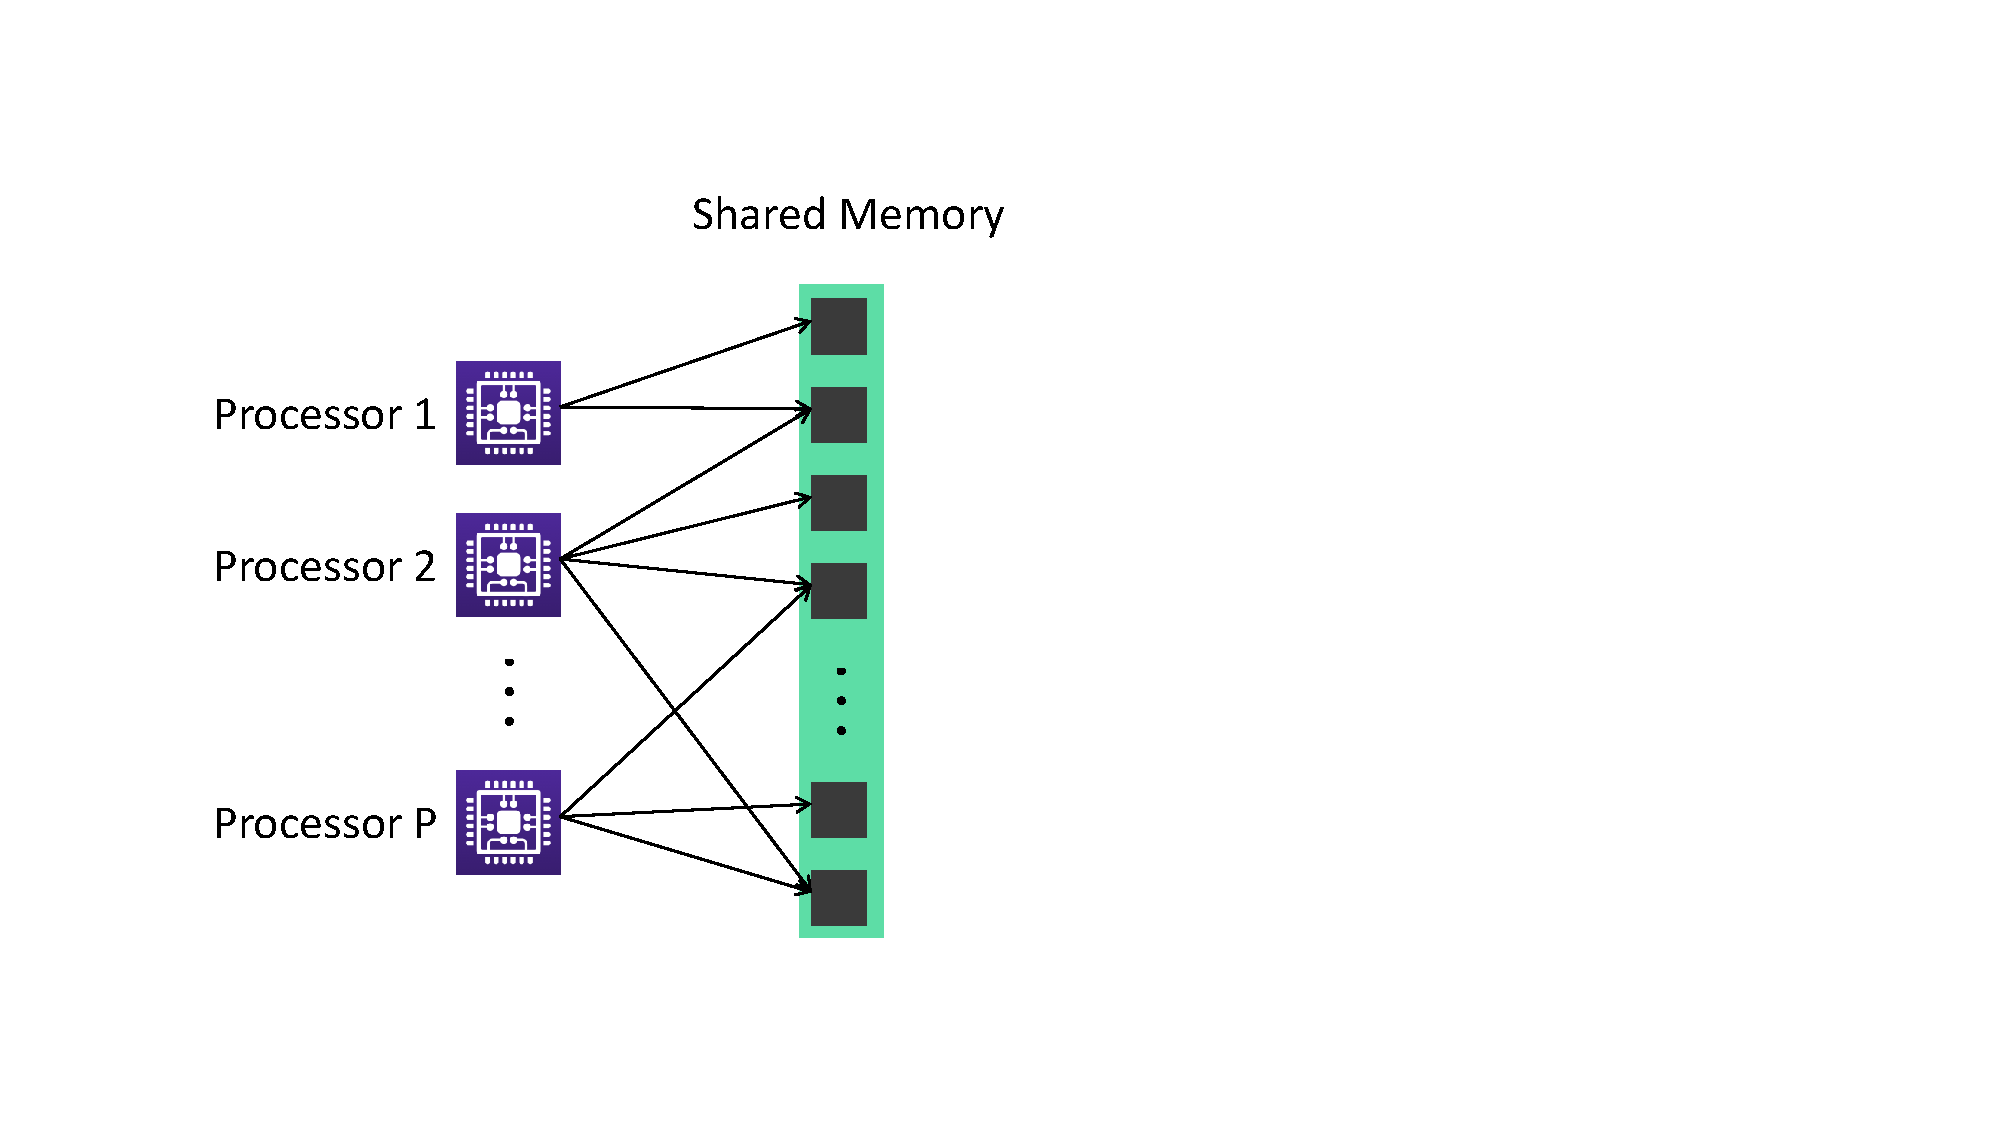
\includegraphics[scale=0.6]{./support/parallel.pdf}
\captionof{figure}{Parallel SGD with an architecture with multiple cores and shared memory.}
\label{fig:parallel}
\end{figure}




\section{Scaling Up SGD}
As shown in Figure~\ref{fig:tradeoff}, a scalable algorithm must excel in accuracy, speed, and parallelizability. While a classic SGD algorithm can deliver accurate solution efficiently (as described in Section~\ref{sec:sgd}), it is inherently serial. We therefore have a technical gap to bridge: \emph{can we parallelize inherently serial algorithms?}

To answer this question, in what follows, we will consider an architecture with multiple cores and shared memory. A parallel version of SGD will store the value of the current parameterization in the shared memory. Each core will read, write the shared memory and perform SGD autonomously in order to update the parameterization, as illustrated by Figure~\ref{fig:parallel}.  Without any coordination among cores, two issues might occur. On one hand, the parameterization read by one core from the shared memory might be \emph{obsolete} as other cores might have computed a newer version of the parameteraization.  On the other hand, a newer version of the parameterization might be \emph{overwritten} by a core that updates the shared memory with a parameterization that is based on \emph{obsolete} information.

To address these issues, a line of research has been leveraging synchronization, with a focus on coordination among cores and applying locks on the parameterization stored in the shared memory during certain stages of the computation. Many coordination and lock based methods suffer from synchronization and communication overhead.  On the contrary, another line of research focuses on the so-called \emph{lock-free} approaches, resulting in the field of asynchronous optimization with literate support dates back to the 1960s \citep{zinkevich2010parallelized, zinkevich2009slow, bertsekas1989convergence, tsitsiklis1986distributed, chazan1969chaotic}. A comparison of these two type of methods is shown in Figure~\ref{fig:asy}.


\begin{figure}
\centering
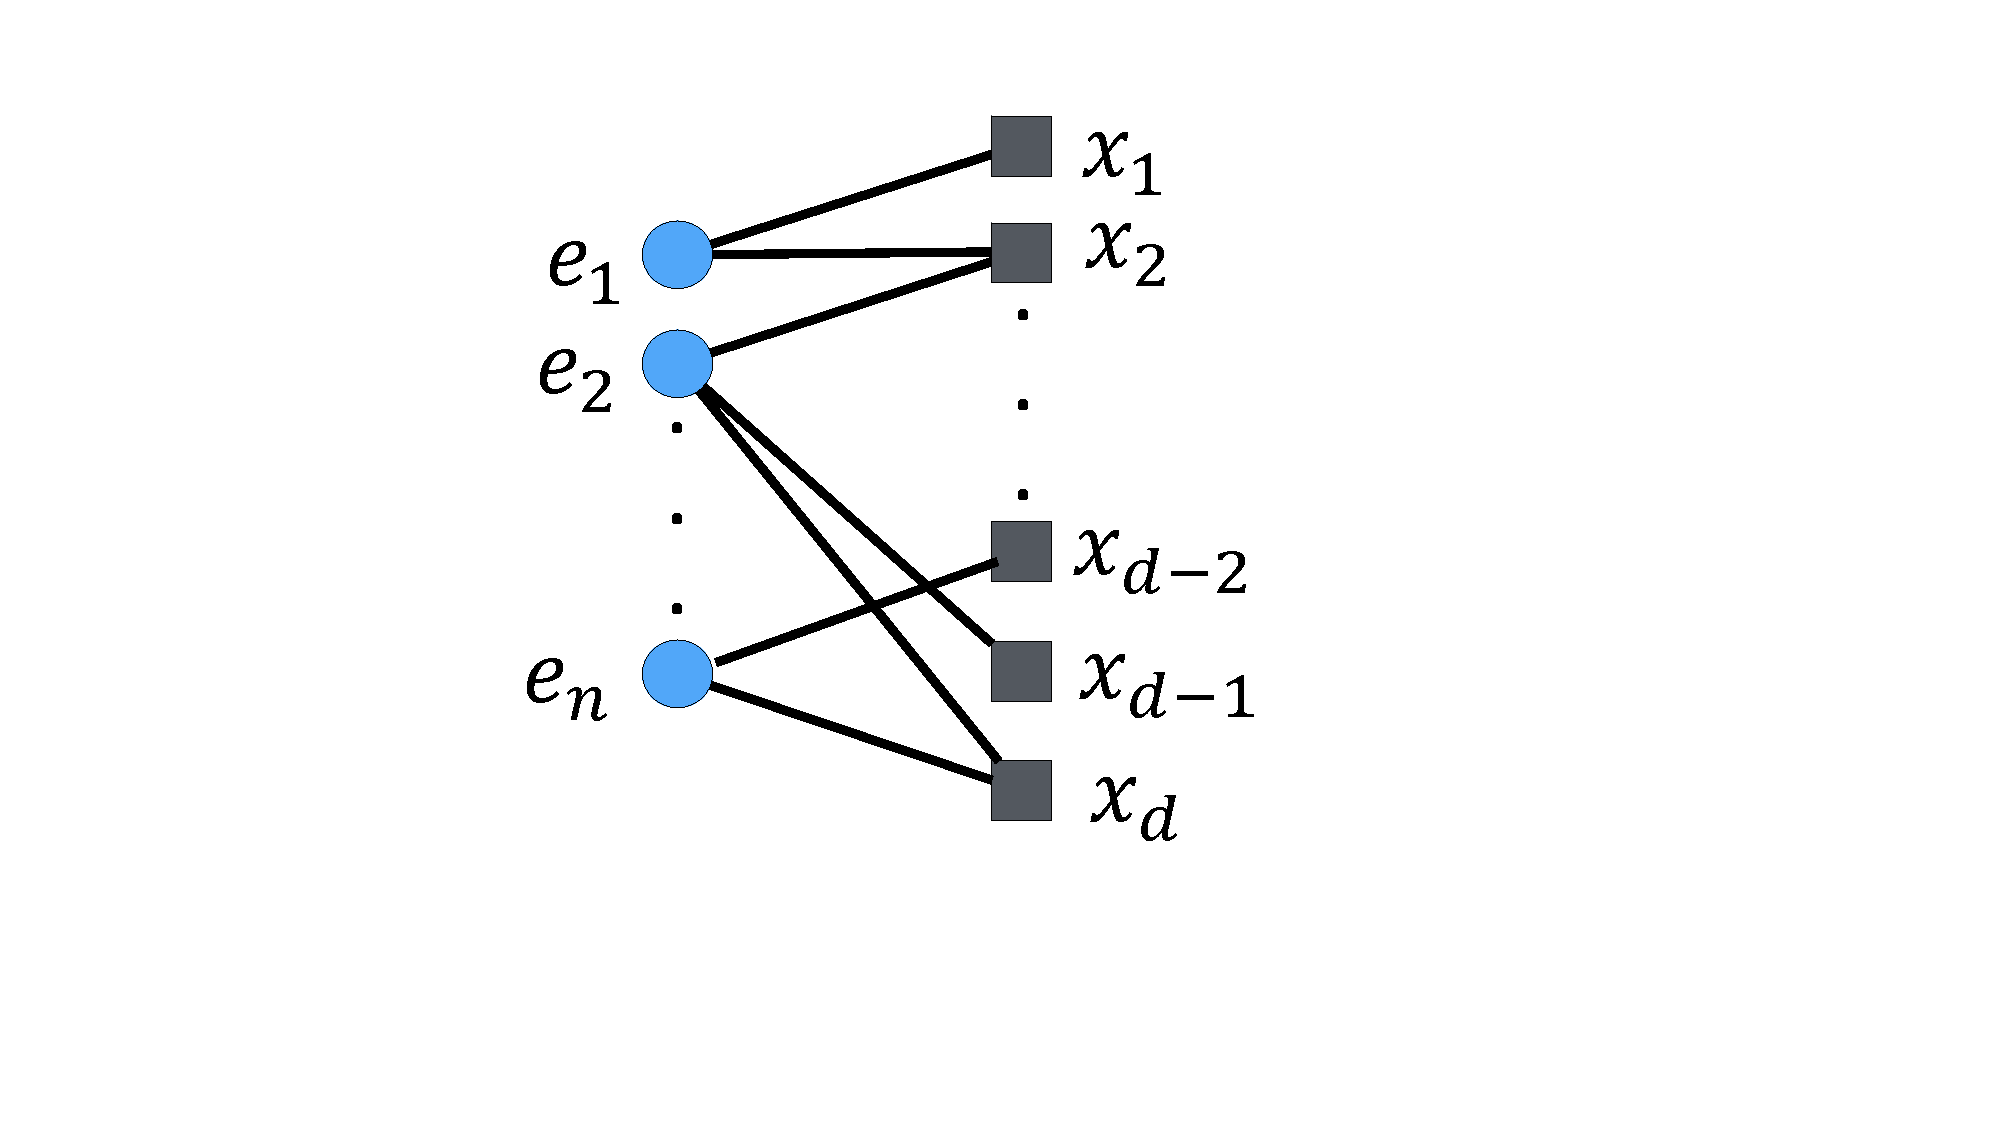
\includegraphics[scale=0.45]{./support/hypergraph.pdf}
\captionof{figure}{A visualization of hypergraph. The set of square nodes represent $V$. Each blue node represents a grouping of indices that constructs the elements in $E$. Since the sample size of the dataset is $n$, the cardinality of $E$ is $n$, i.e.~$\notate{card}E=n$. Since the dimension of the parameterization is $d$, we have $\notate{card}V = d$.}
\label{fig:hypergraph}
\end{figure}

\begin{figure}
\centering
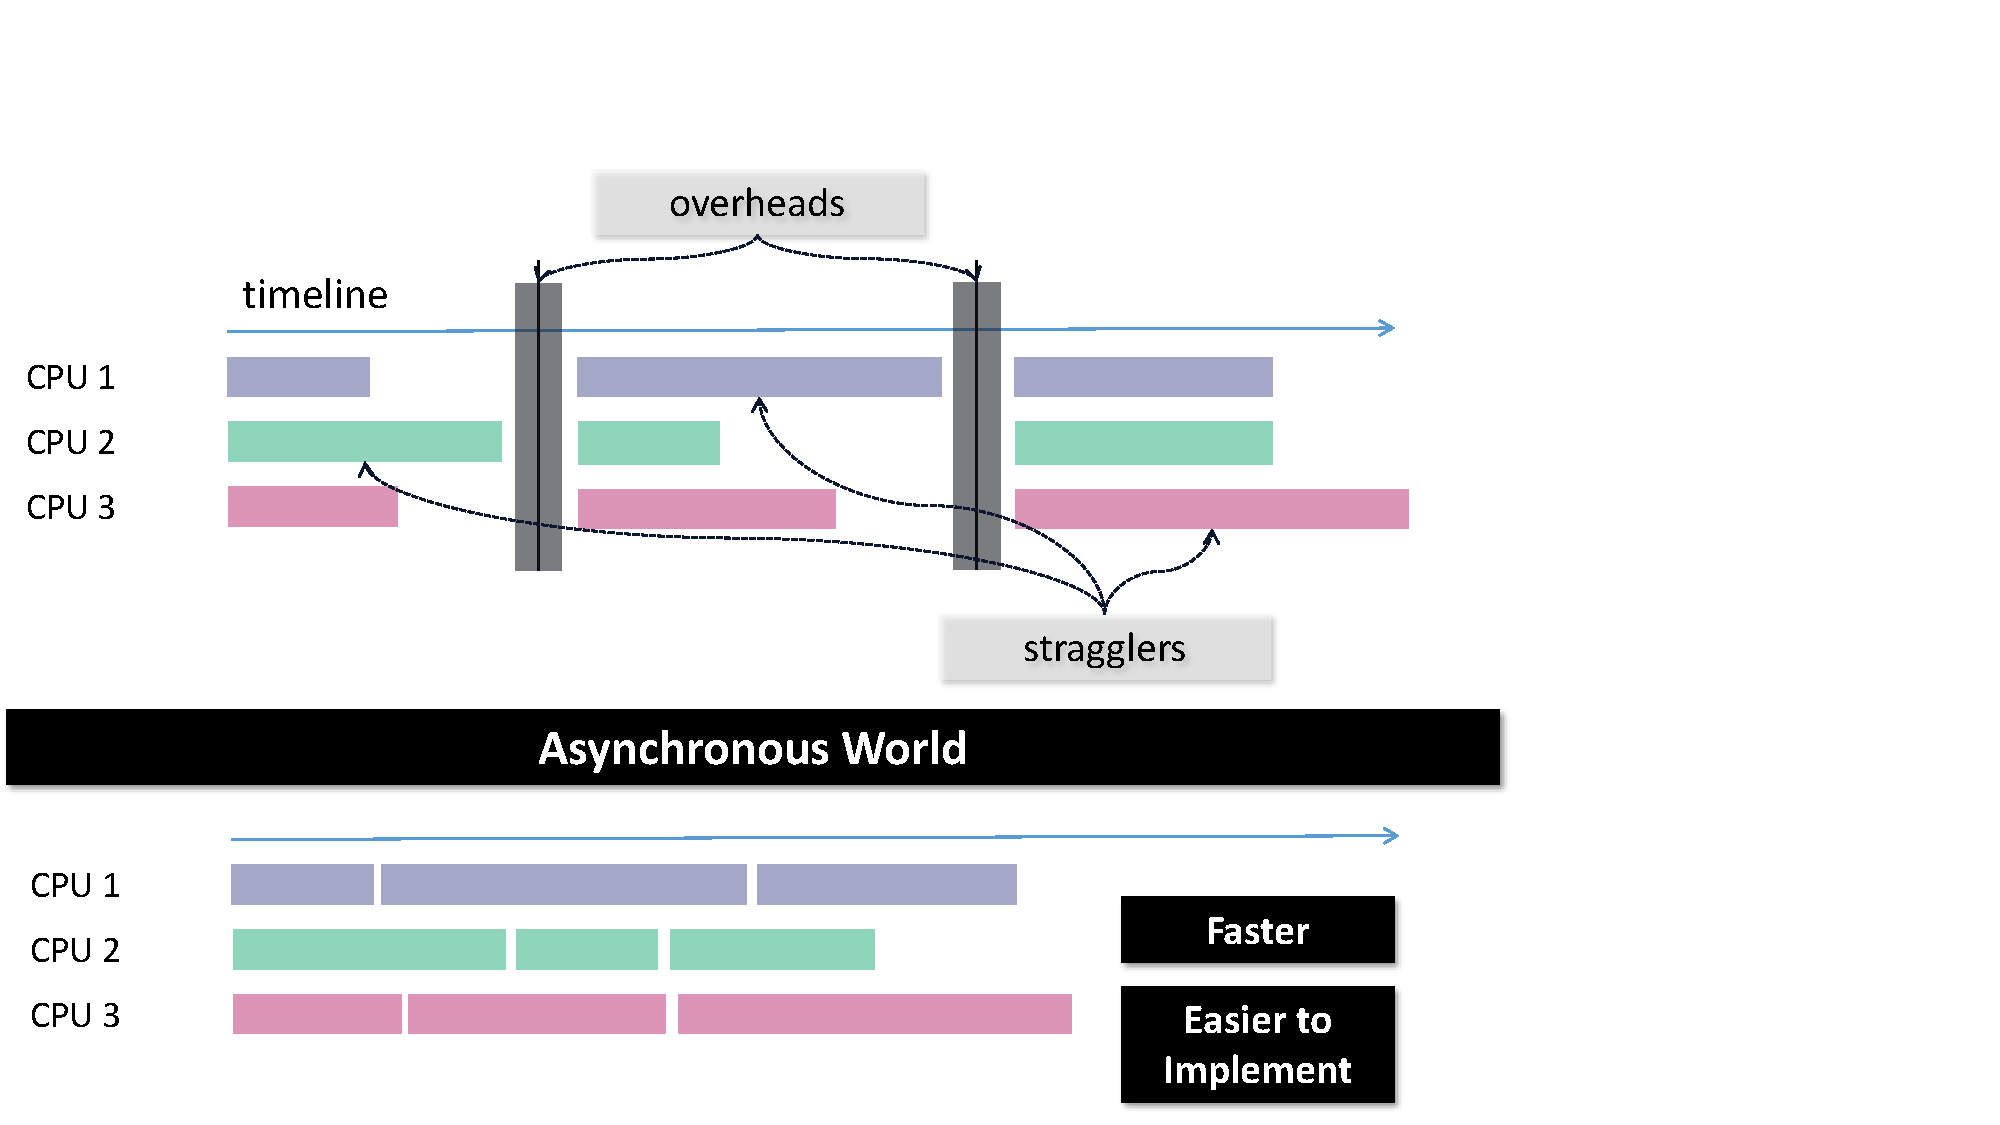
\includegraphics[scale=0.6]{./support/asy.pdf}
\captionof{figure}{A case against synchronization.}
\label{fig:asy}
\end{figure}

\begin{algorithm}[t]
\caption{\textsc{HogWild!}}
\label{alg:hw}
\begin{algorithmic}[1]
\Require $\mathcal{D}$.
\Ensure $x$.
\State Initialize $x$ in shared memory.
\State Compute $E$ from $\mathcal{D}$.
\For{$i \in \curly{1,2,\cdots,p}$} \textbf{in parallel}
\While{true}
\If{Stopping criteria satisfied}
\State \textbf{break}.
\EndIf
\State Sample $j \in \curly{1,2,\cdots,n}$.
\State Get $x$ from shared memory, choose step length $\gamma$.
\State Compute $f_j(x;e_j)$, and $\grad f_j(x;e_j)$.
\label{step:grad}
\For{$k \in e_j$}
\State $x_k \leftarrow x_k - \gamma \grad_k f_j(x;e_j)$.
\EndFor
\EndWhile
\EndFor
\end{algorithmic}
\end{algorithm}


\section{Lock-Free Parallelization of SGD}
In many machine learning problems that can be solved by SGD, the value of $f_i(x)$, given $i \in \curly{1,2,\cdots,n}$, is usually dependent only on a handful of components in $x$, while the dimension of $x$ can be relatively high. \cite{recht2011hogwild} exploit this kind of \emph{sparsity} and propose an algorithm called 
\textsc{HogWild!}, which is a lock-free parallelization of SGD with \emph{provable} optimizational guarantee under the aforementioned sparsity assumption.

Let $e_i\subseteq \curly{1,2,\cdots,n}$ be a subset of indices on which the value of $f_i(x)$ depend. i.e.~given $e_i$ and a subvector $x_{e_i}$, which is constructed by the components of $x$ indexed by $e_i$, the value of $f_i(x)$ is completely determined  without knowing the values of other components that are not indexed by $f_i(x)$. We denote $E = \curly{e_i \mid i\in \curly{1,2,\cdots,n}}$, and $V = \curly{x_1,x_2,\cdots,x_d}$. We can use a \emph{hypergraph}\footnote{A hypergraph is a generalization of a graph in which an edge can join any number of vertices.}, denoted as $(V,E)$, to represent the dependency between the value of $f_i(x)$ and the components of $x$. Figure~\ref{fig:hypergraph} visualizes a hypergraph. The set of square nodes represent $V$. Each blue node represents a grouping of indices that constructs the elements in $E$. For example, $e_1 = \curly{1,2}$. Therefore, $f_1(x)$, which is the value of the loss function evaluated on the first data point in the dataset, is dependent only on the first component and the second component of the parameterization. With these notation, we can rewrite the objective function as:
\begin{equation*}
\arg\min_{x\in\mathbb{R}^d} \sum_{i=1}^n f_i(x;e_i),
\end{equation*}
where $f_i(x;e_i)$ emphasizes the fact that $f_i$ is only dependent on the components of $x$ indexed by $e_i$. We use $\mathcal{D}$ to denote the dataset. The algorithm of \textsc{HogWild!} is given in Algorithm~\ref{alg:hw}. Note that in Step~\ref{step:grad}, since $f_i(x;e_i)$ is only dependent on $e_i$, $\grad f_i(x;e_i)$ is also only dependent on $e_i$. 

When $e_i \cap e_j = \emptyset$, where $i\ne j$, and $i,j\in \curly{1,2,\cdots,n}$, performing SGD in parallel using $f_i(x)$ and $f_j(x)$ in different cores respectively is equivalent to performing the two iterations in a serial fashion. However, when $e_i \cap e_j \ne \emptyset$, performing SGD in parallel will introduce conflicts. Nonetheless, with the sparsity assumption, one can show that the occurrences of such conflicts are rare and the convergence of \textsc{HogWild!} will not be hindered much by conflicts, resulting in \emph{linear} speedup with the number of processors on many common sparse learning problems. 

\section{Convergence Analysis}
Due to parallelization, the theoretical convergence analysis of \textsc{HogWild!} is incompatible with the convergence analysis of SGD. To prove that Parallel SGD and Serial SGD have similar convergence rates for given number of samples, new theoretical general framework are needed for asynchronous lock-free Algorithms.  Two measures of performance are of interest in the analysis:
\begin{gather*}
\text{speedup} = \frac{\text{Time of serial } \mathcal{A} \text{ to accuracy } \epsilon}{\text{Time of parallel } \mathcal{A} \text{ to accuracy } \epsilon},\\
\text{worst case speedup} = \frac{\text{bound on number of iterations of SGD to } \epsilon}{\text{bound on number of interations of Parallel SGD to } \epsilon}.
\end{gather*}

In the next lecture, we will talk about challenges arise in the convergence analysis of asynchronous lock-free Algorithms in details. 

\section*{References}
\begingroup
\renewcommand{\chapter}[2]{}
\bibliography{15refs}
\endgroup

\end{document}
